\Cref{sec:fitting_mbc,sec:background_subtraction} introduced the fitting procedure and \BB background subtraction.
Together with the optimal selections from \Cref{sec:final_optimisation}, this fully defines the analysis strategy from the Belle~II simulated datasets to the \BtoXsgamma spectrum.
However, the defined fitter has to be validated in simulation to give an unbiased estimation of \BtoXsgamma events, with a good resoltion and signal efficiency.
The studies in this Section will show such results.

\subsection{Validation of \texorpdfstring{\Mbc}{Mbc} fit on reduced samble size}\label{sec:mbc_fit_validation_misreconstructed}

The results that were shown in \Cref{fig:mc_fit_yield_comparisons} only provided results for fitting 1.6~\invab -- a dataset about an order of magnitude larger than is expected in the case of this analysis.
Therefore, the generic \MC dataset is pseudorandomly split into 10 smaller subsets, corresponding to 160~\invfb, and each of them are fitted independently.
The choice of 160~\invfb, rather than 190~\invfb which is the sample size of the Belle~II data used in the analysis, is due to anticipated data-simulation differences.
\todo[inline]{see XXX and next paragraph performed where?}
Indeed, a 190~\invfb dataset should correspond to roughly 160~\invfb in simulation due to differences in tag-\B reconstruction efficiency.

The resulting 10 fits and the estimated $\mathcal{N}_{CB}$ corresponding to each \EB bin are shown in \Cref{fig:extracted_validation_mc}.
The expected number of events in each fit is always equal to one tenth of that in the total generic \MC dataset.
It can be observed that all data points, and their average, are statistically compatible with the expectation.
These results indicate, that despite using a 10 times larger dataset to define the \PDF{s}, this \Mbc fit model produces reliable and stable results.
Further tests, particularly a test ensuring that the fitter is unbiased, are performed later.

\begin{figure}[htbp!]
    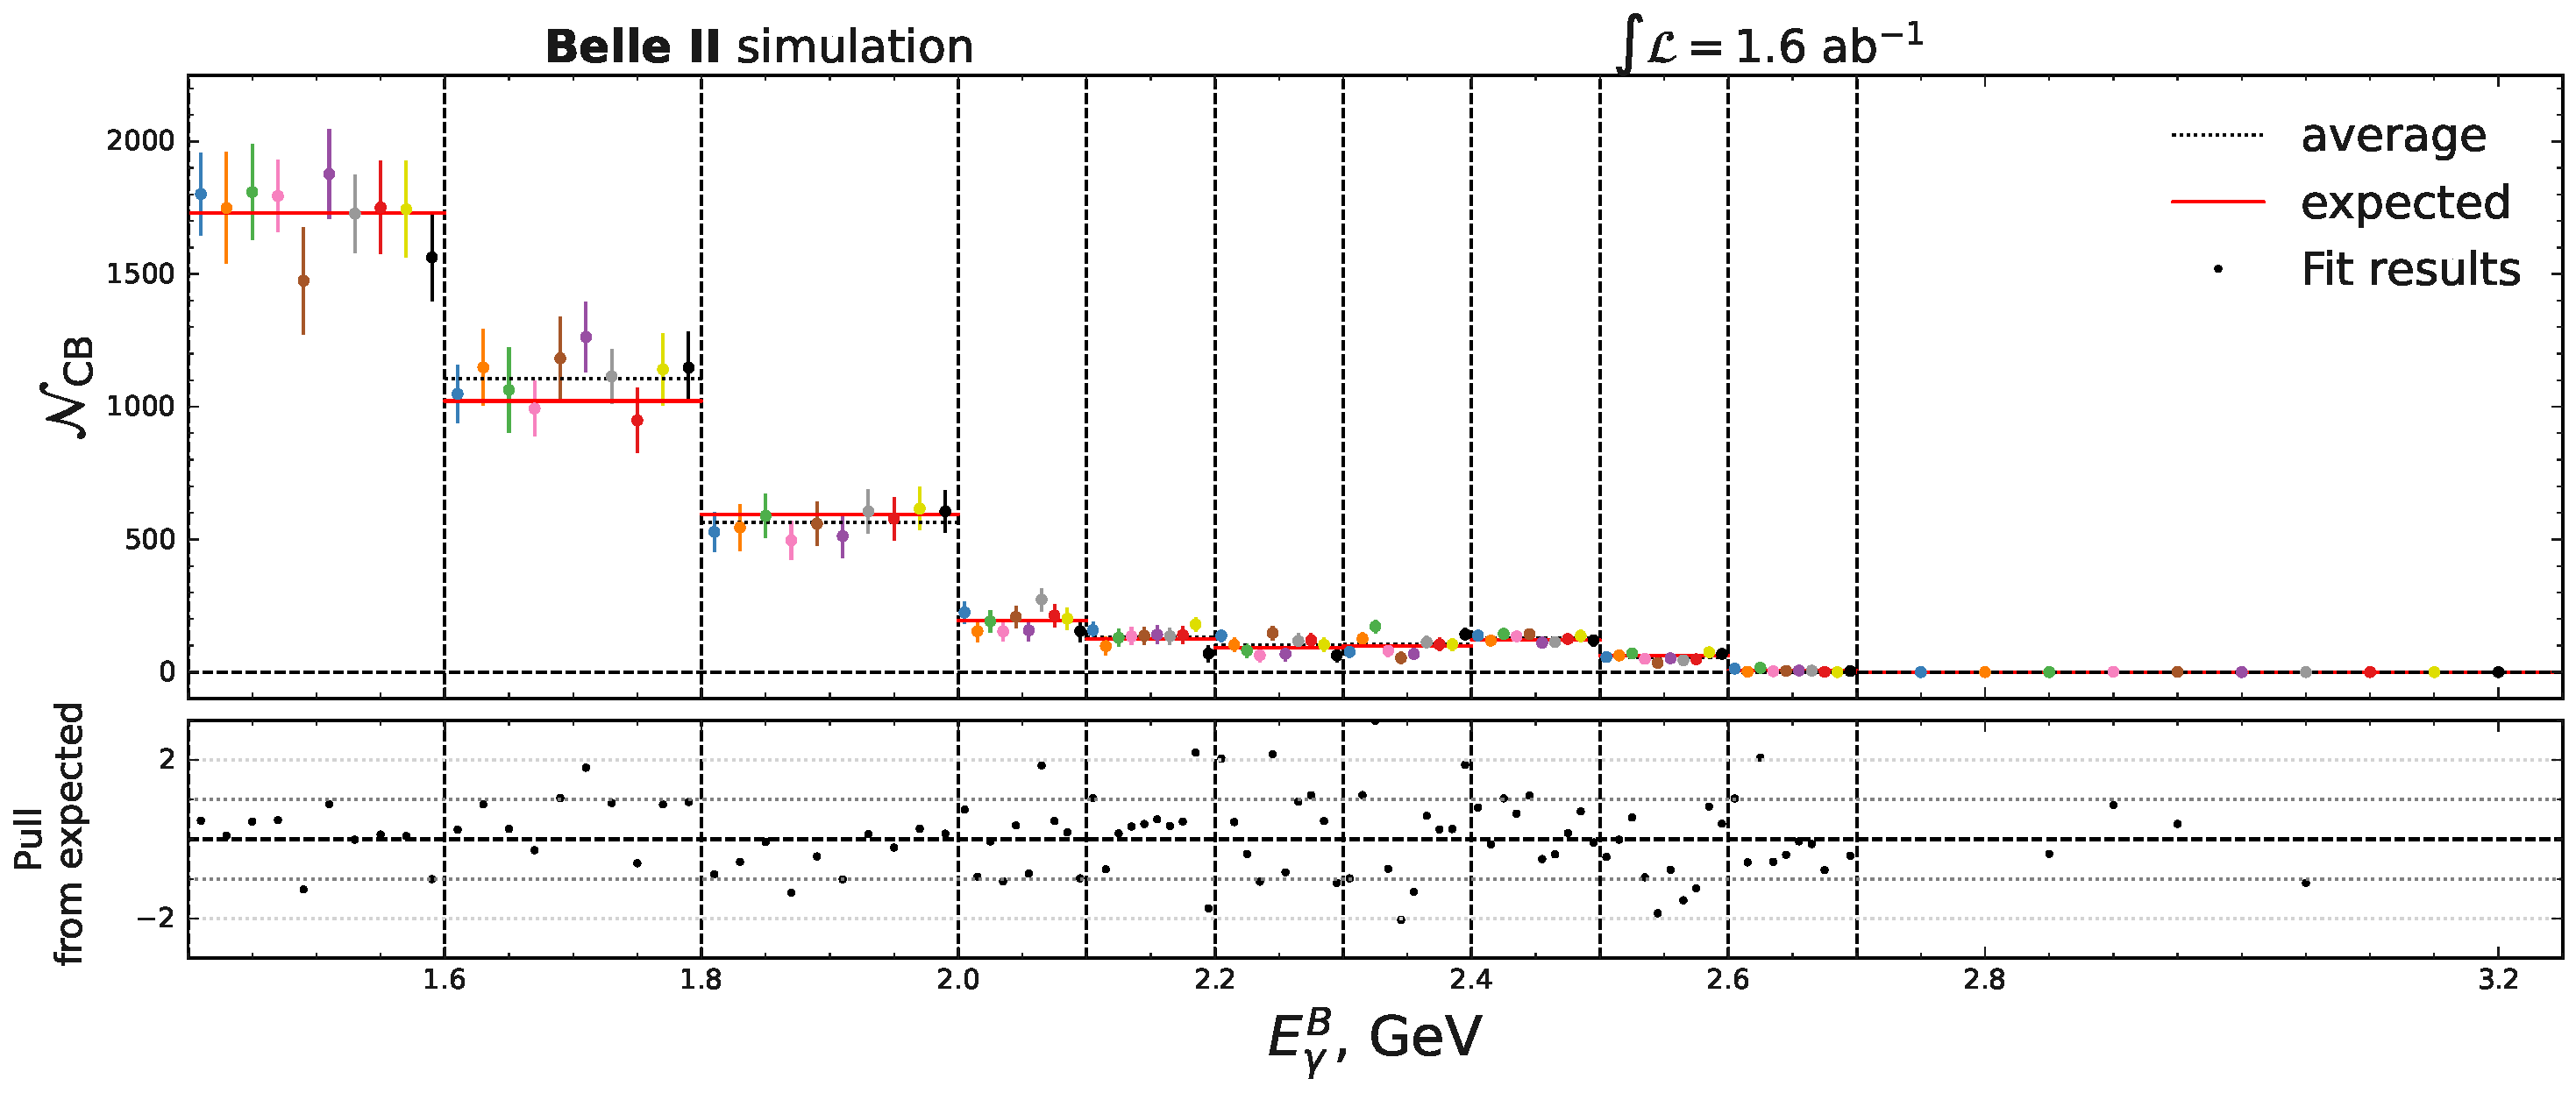
\includegraphics[width=0.9\textwidth]{figures/mc_validation/extracted_signal_generic_mc.pdf}
    \caption{\label{fig:extracted_validation_mc}The estimated $\mathcal{N}_{CB}$ values from fits on one tenth of generic \MC, corresponding to 160~\invfb of simulation.
    The dashed lines represent different \EB bins, each bin showing one data point corresponding to a simultaneous fit of all \EB bins.
    The dotted lines show the average of all 10 points in each bin, whereas the full lines show the number of good tag-\B events in the original 1.6~\invab dataset, scaled down 10 times (`expected').
    The subpanels show the pull of each datapoint from the expected number of events.
    These results show that the fit is able to extract a result on a dataset that is an order of magnitude smaller.
    }
\end{figure}

\subsection{Validation of subtraction of remaining-\texorpdfstring{\BB}{BB} background}\label{sec:background_subtraction_validation_mc}

The strategy to extract the \BtoXsgamma photon energy spectrum and suppress the remaining \BB background was laid out in \Cref{sec:background_subtraction}.
In particular, full generic \MC dataset is modified, such that no-\BtoXsgamma events are present in it.
Then, the \Mbc fit discussed in \Cref{sec:fitting_setup} is performed.
To test that this procedure is viable, the subtraction is performed for the results shown in \Cref{fig:extracted_validation_mc}.
Although the 10 fits are performed on 160~\invfb datasets, the background subtraction is done with a 1.6~\invab dataset.
Therefore, the statistical uncertainty from the fit on the smaller dataset is dominating.
The subtracted result is shown in \Cref{fig:subtracted_validation_mc}.

\begin{figure}[htbp!]
    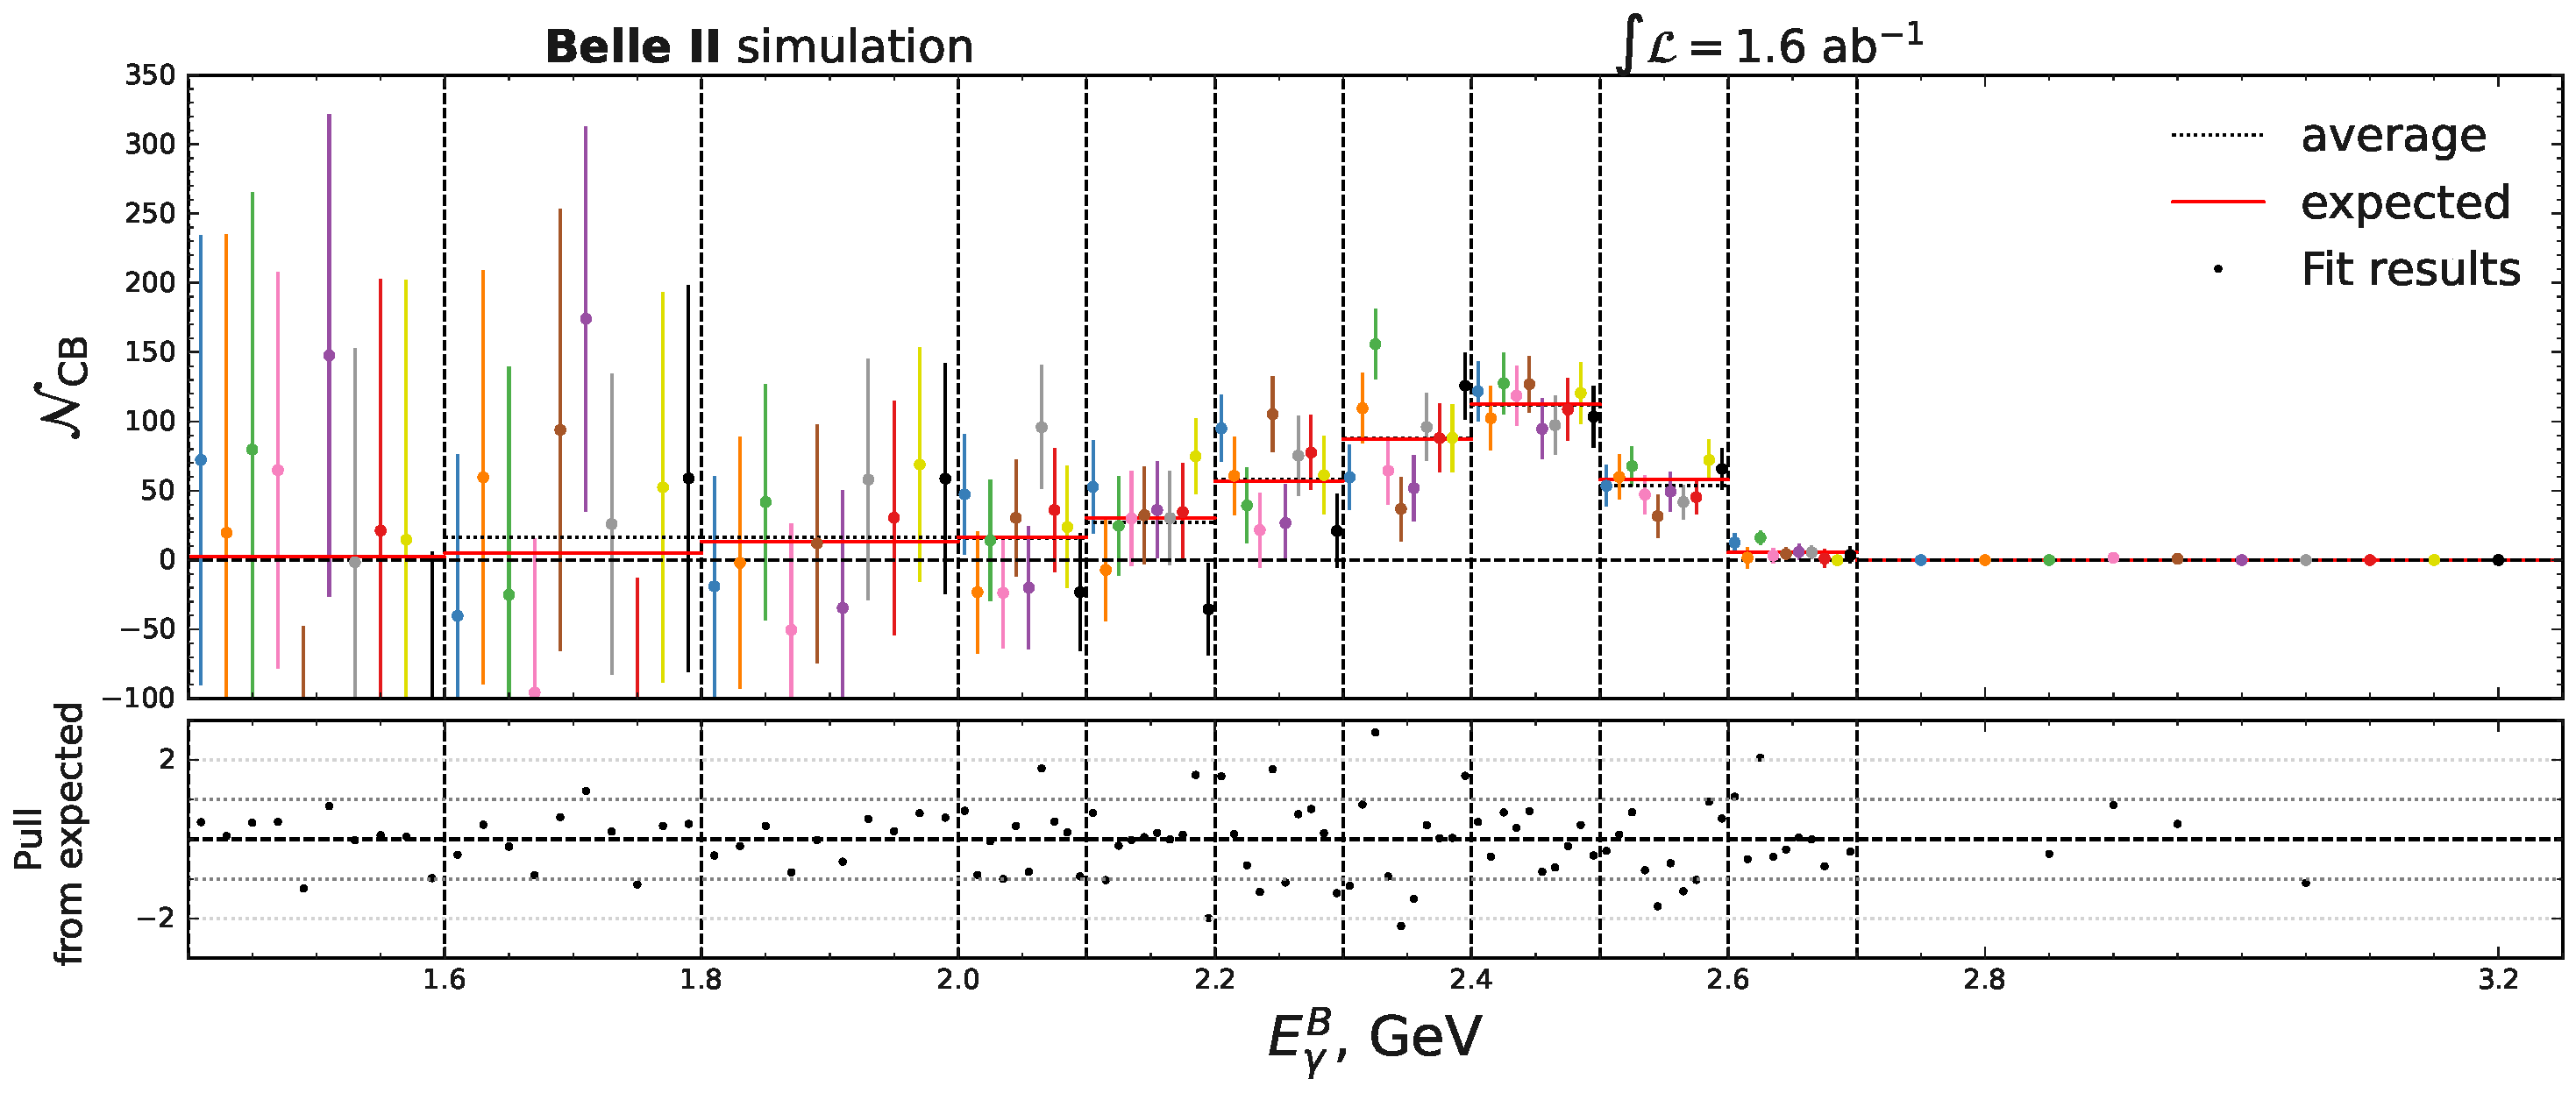
\includegraphics[width=0.9\textwidth]{figures/mc_validation/subtracted_signal_generic_mc.pdf}
    \caption{\label{fig:subtracted_validation_mc}
    The estimated $\mathcal{N}_{CB}$ with subtracted background, based on the \Cref{eq:background_subtraction}.
    The values before \BB-background subtraction are shown in a corresponding \Cref{fig:extracted_validation_mc}.
    To ensure that a minimal statistical background subtraction uncertainty is introduced, the full 1.6~\invab dataset is chosen to subtract the background.
    The uncertainties of each data point are those of the \Mbc fit on the background dataset and on the tested subset, added in quadrature.
    }
\end{figure}

The 1.6~\invab dataset and the 160~\invfb subsets are largely correlated, therefore the result has a smaller spread than one might expect from a unit Gaussian, based on the statistical ucnertainty provided by the fitter.
However, the purpose of this test is to showcase that the setup is able to extract values that are statistically compatible with the original dataset.
The results showcased in \Cref{fig:extracted_validation_mc,fig:subtracted_validation_mc} clearly show that the central values of the \EB spectrum extracted follow the number of \BtoXsgamma events in the dataset.
In this section so far, no particular modelling of \BtoXsgamma spectrm has been assumed.
In fact, following the tests from \Cref{fig:mc_fit_yield_comparisons}, it is clear that the analysis is \textit{so far} signal-model independent, as no direct assumptions have been made thus far.
On the other hand, following the setup that is taken to remove \BB backgrounds after the \Mbc fit, the analysis is heavily background-model dependent.
For this reason, special emphasis will be put on testing the \textit{background} description validation, as opposed to signal validation in later chapters XXXX.
\todo[inline]{later chapter xxxx}

\subsection{Closure test of the \texorpdfstring{\Mbc}{Mbc} fitter}\label{sec:closure_test}

If the uncertainties estimated by a fitter are correct, then fitting pseudodata sets generated from \PDF{s} fitted on test data must yield statistically compatible results.
This verifies two important aspects of the fitter:
\begin{itemize}
    \item the estimated parameter central values of the fitter are reproduced, when fitting a statistically equivalent dataset;
    \item the estimated parameter central values of the fitter are distributed accordingly to the uncertainties that the fitter provides.
\end{itemize}

More concisely, the pull distribution of an unbiased fitter, in this case calculated as:
\begin{equation}\label{eq:toy_pull}
    \mathrm{pull} = \frac{\mathcal{N}\times \mathrm{scale} - \mathcal{N}^{\mathrm{pseudo}}}{\mathrm{fit~error}},
\end{equation}
must be described by a unit Gaussian (assuming the central limit theorem is applicable for the psuedodata sample size).
In the case of this analysis, $\mathcal{N}_{\mathrm{CB}}$ is the estimated number of good tag-\B mesons in the generic-\MC sample.
The uncertainty, $\mathrm{fit~error}$ is a corresponding uncertainty, in this analysis estimated by the \texttt{HESSE} method.
On the other hand, $\mathcal{N}^{\mathrm{pseudo}}_{\mathrm{CB}}$ is a randomly sampled dataset that follows the \PDF{s} fitted on the generic-\MC dataset.
The $\mathrm{scale}$ is used to equate the sample size between the sampled and total simulated dataset.
Tests of this type are known as \textit{closure tests} is statistics and allow to verify that the central values reproduced by the fitter fluctuate as indicated by the \PDF uncertainties.

The closure test in this analysis is done on pseudodata sets of equivalent size as the Belle II collected data.
First, 1000 pseudodata sets equivalent to $\mathrm{160~\invfb}$ are sampled from the \PDF that was fitted in \Cref{fig:primary_full_fits}.
Since in all of the cases $\mathcal{N}_{\mathrm{CB}}$ and $\mathrm{fit~error}$ are known exactly, the \Mbc fitter is used on the pseudodata set, and a $\mathrm{pull}$ is calculated based on \Cref{eq:toy_pull}.
The pull distribution for every \EB bin are shown in \Cref{fig:pull_distributions}.

\begin{figure}[htbp!]
    \centering
    \subcaptionbox{\label{fig:pulls_1p4to1p6}}{
        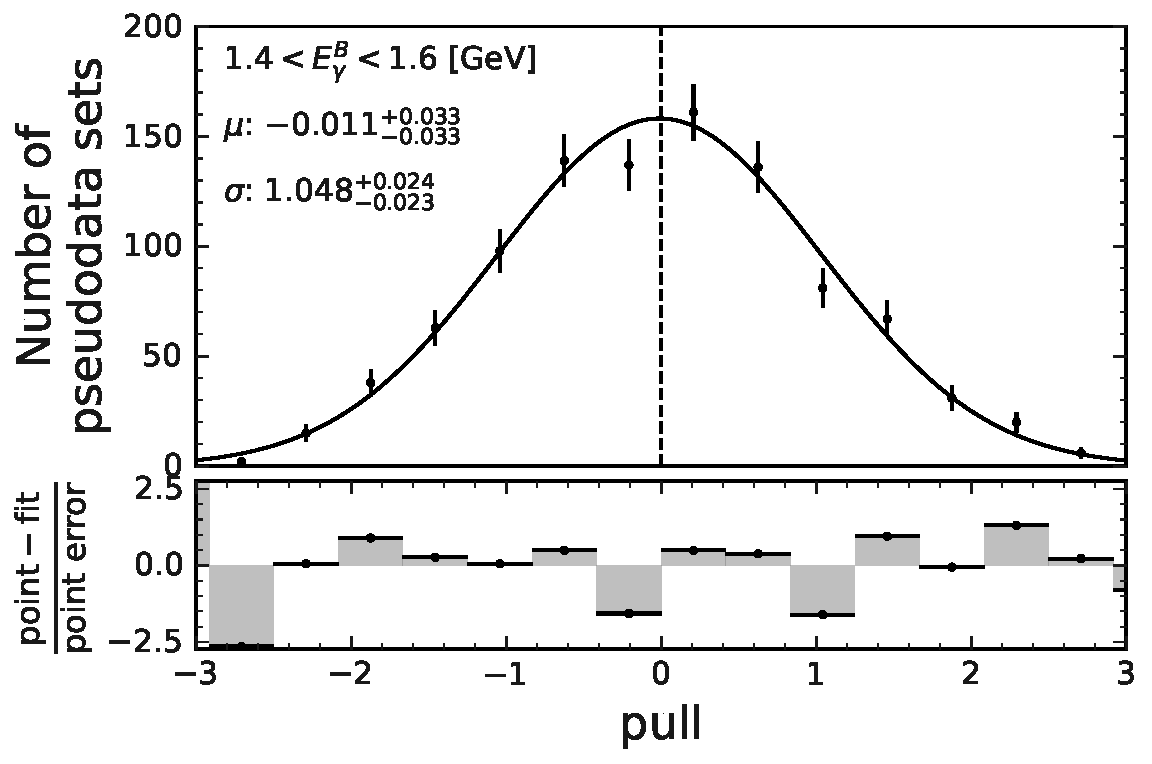
\includegraphics[width=0.22\textwidth]{figures/mc_validation/toy_study/fits_of_pulls_1p4to1p6.pdf}
    }
    \subcaptionbox{\label{fig:pulls_1p6to1p8}}{
        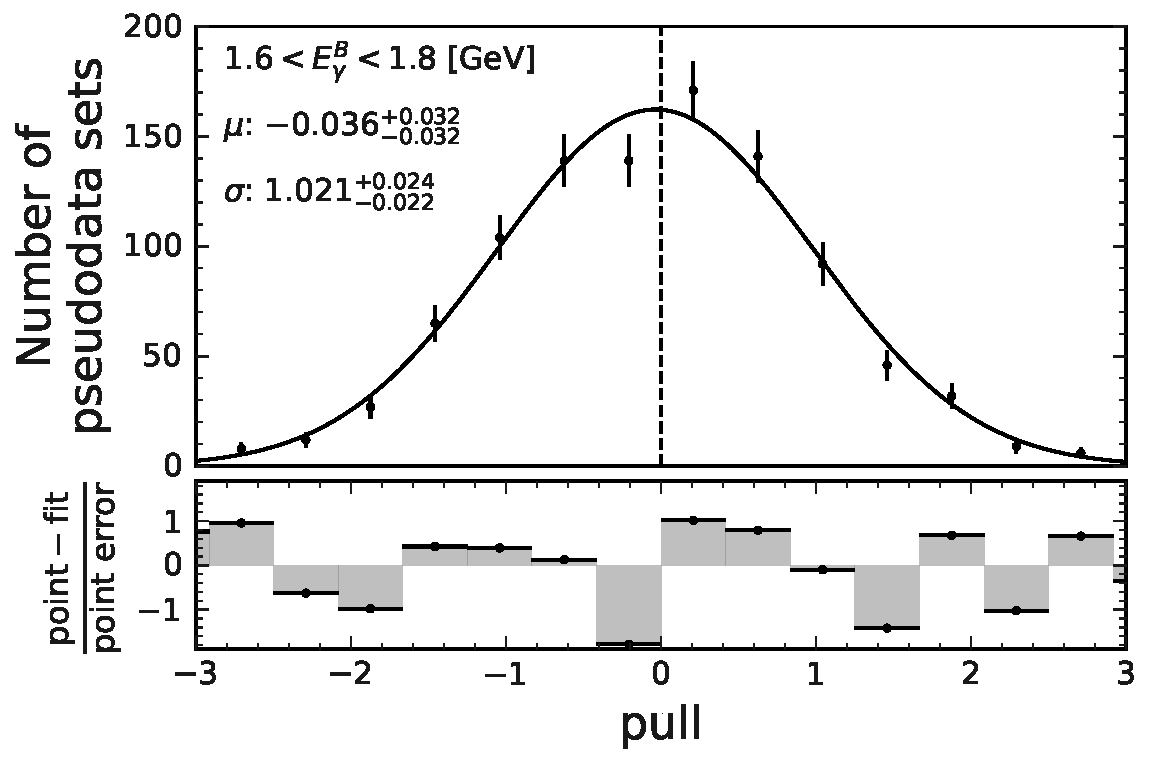
\includegraphics[width=0.22\textwidth]{figures/mc_validation/toy_study/fits_of_pulls_1p6to1p8.pdf}
    }
    \subcaptionbox{\label{fig:pulls_1p8to2p0}}{
        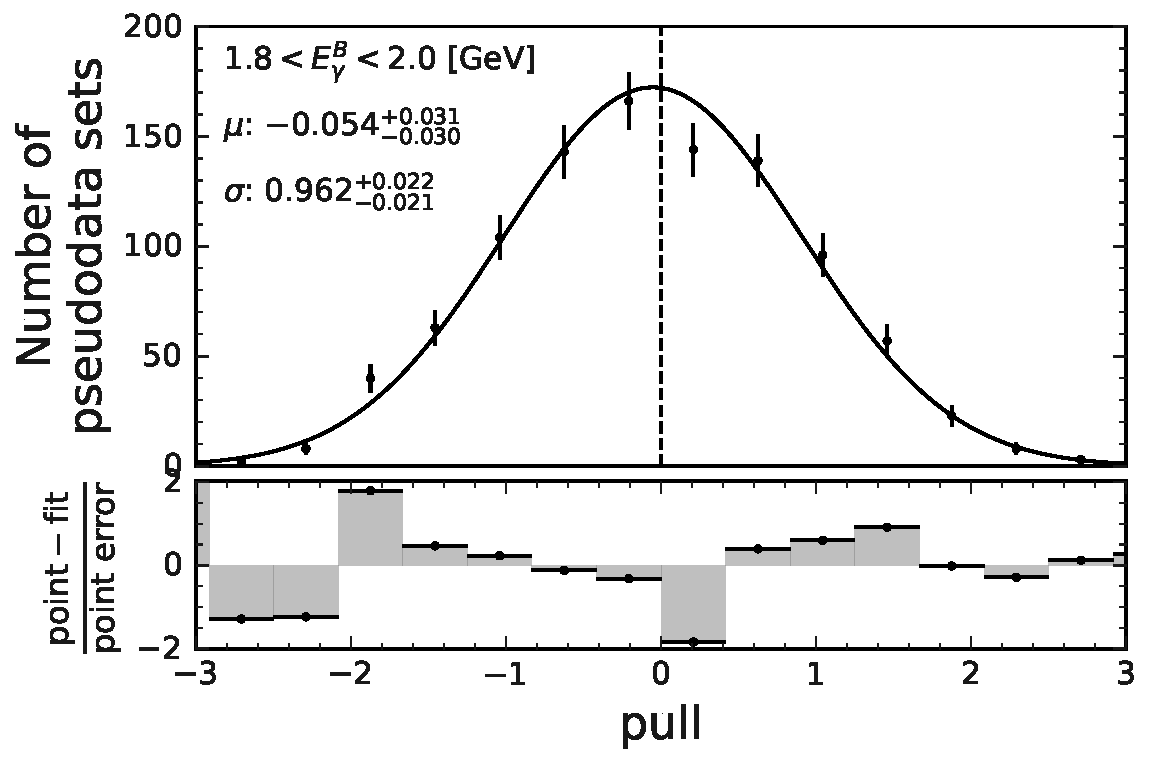
\includegraphics[width=0.22\textwidth]{figures/mc_validation/toy_study/fits_of_pulls_1p8to2p0.pdf}
    }
    \subcaptionbox{\label{fig:pulls_2p0to2p1}}{
        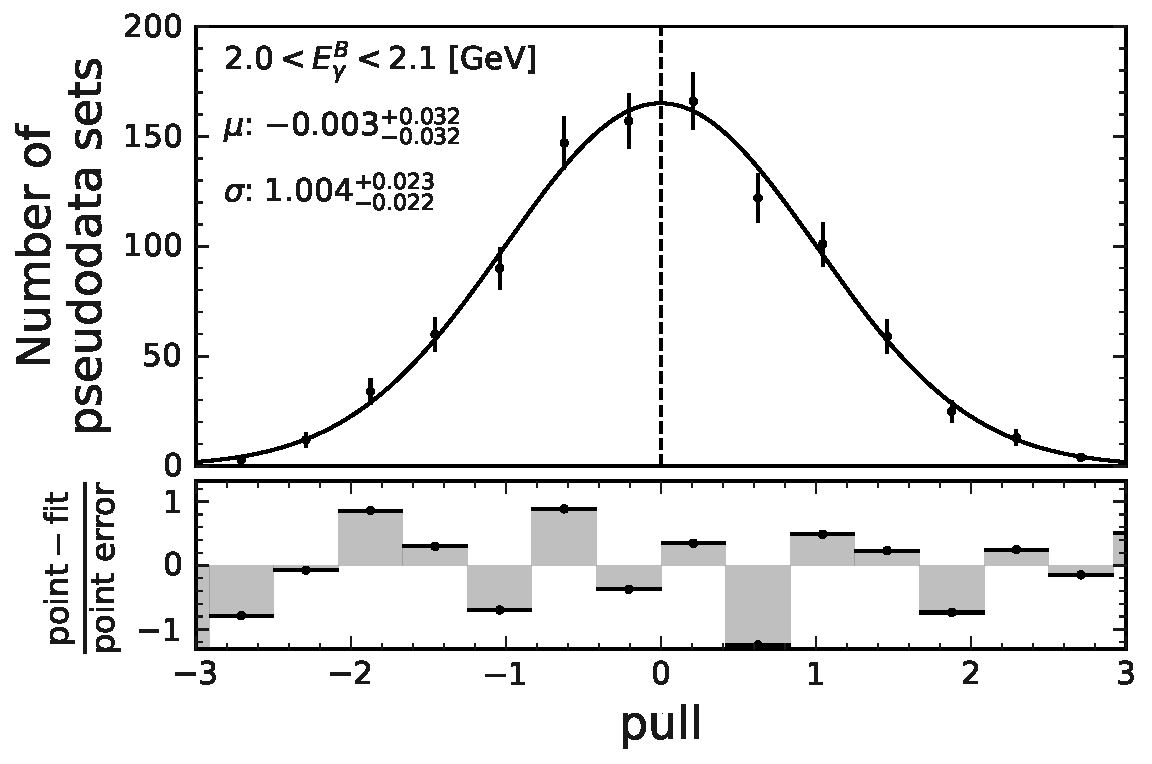
\includegraphics[width=0.22\textwidth]{figures/mc_validation/toy_study/fits_of_pulls_2p0to2p1.pdf}
    }
    \subcaptionbox{\label{fig:pulls_2p1to2p2}}{
        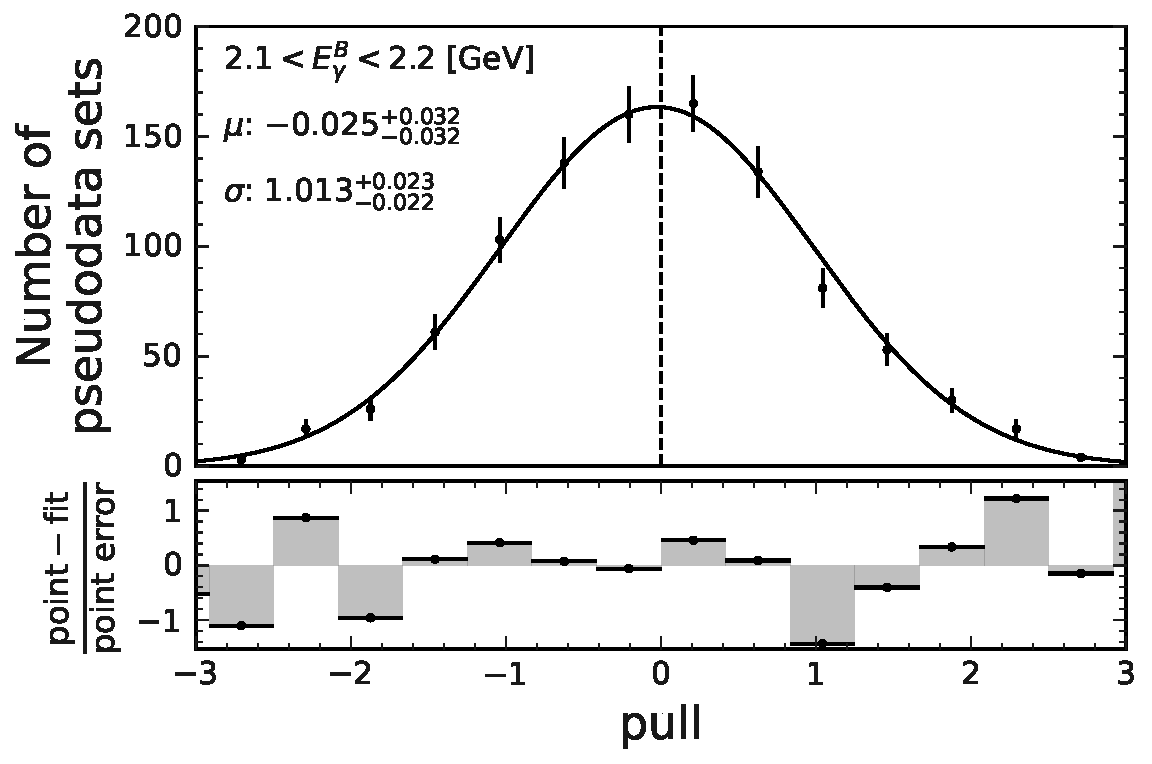
\includegraphics[width=0.22\textwidth]{figures/mc_validation/toy_study/fits_of_pulls_2p1to2p2.pdf}
    }
    \subcaptionbox{\label{fig:pulls_2p2to2p3}}{
        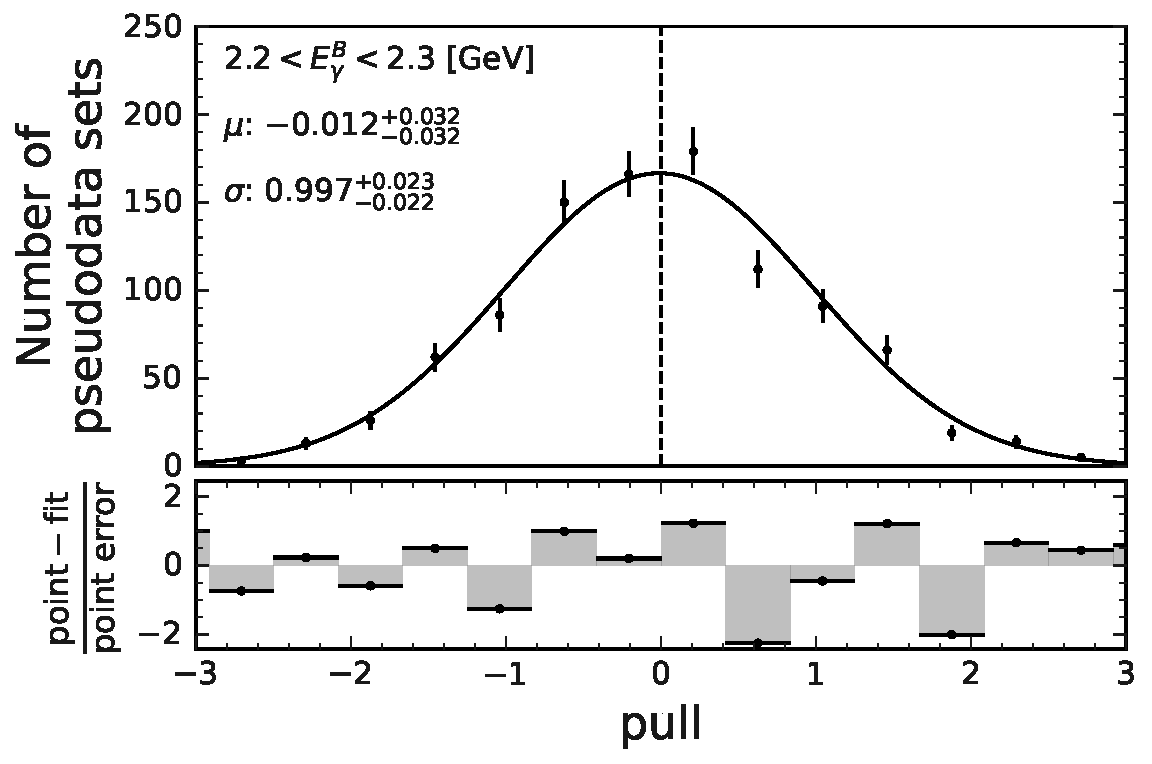
\includegraphics[width=0.22\textwidth]{figures/mc_validation/toy_study/fits_of_pulls_2p2to2p3.pdf}
    }
    \subcaptionbox{\label{fig:pulls_2p3to2p4}}{
        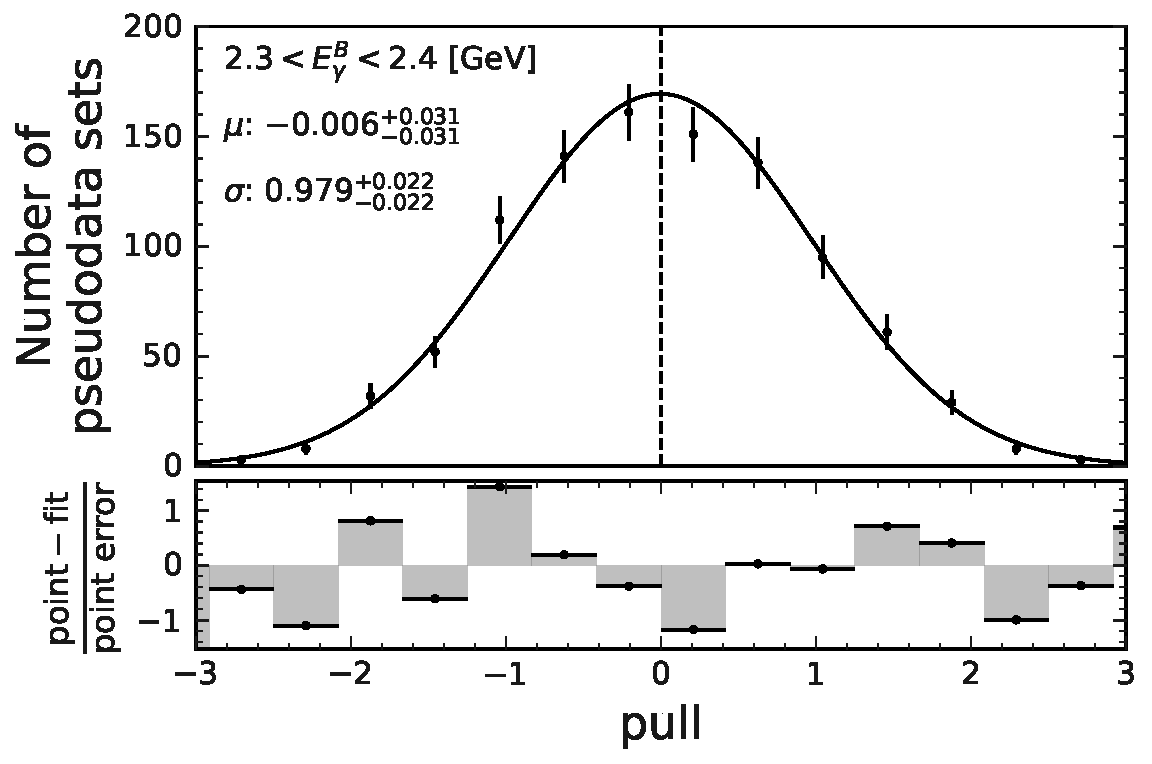
\includegraphics[width=0.22\textwidth]{figures/mc_validation/toy_study/fits_of_pulls_2p3to2p4.pdf}
    }
    \subcaptionbox{\label{fig:pulls_2p4to2p5}}{
        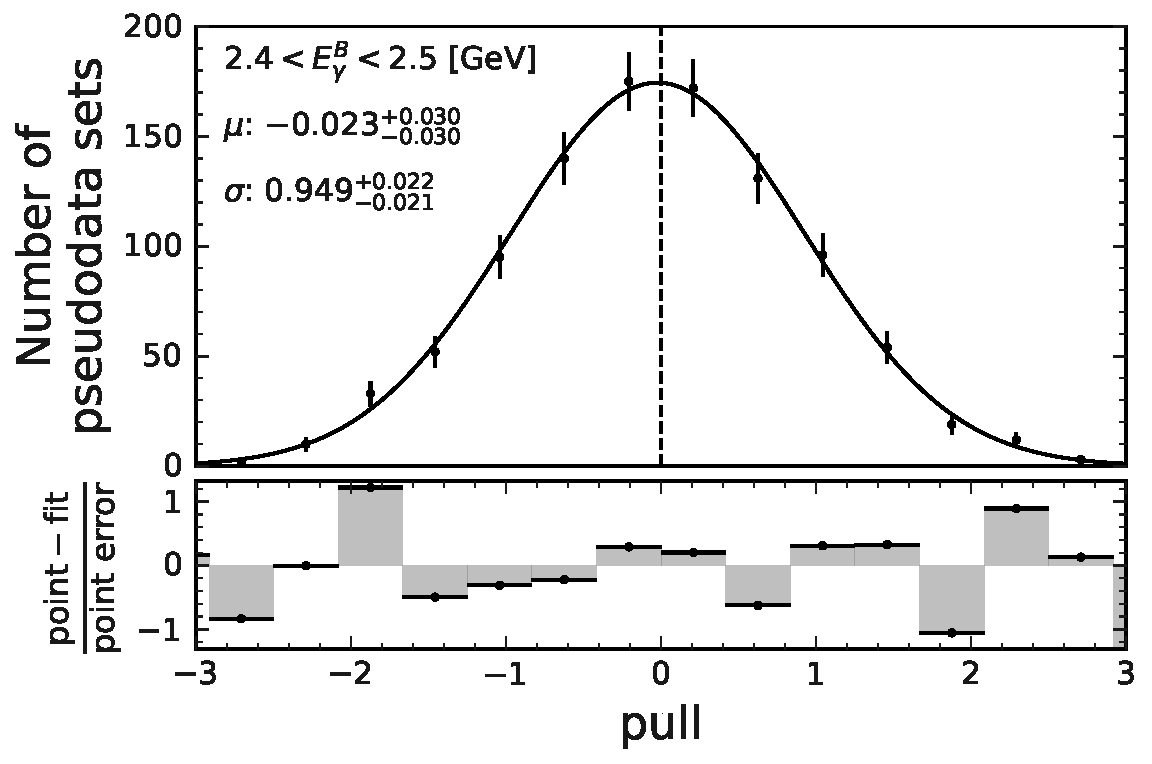
\includegraphics[width=0.22\textwidth]{figures/mc_validation/toy_study/fits_of_pulls_2p4to2p5.pdf}
    }
    \subcaptionbox{\label{fig:pulls_2p5to2p6}}{
        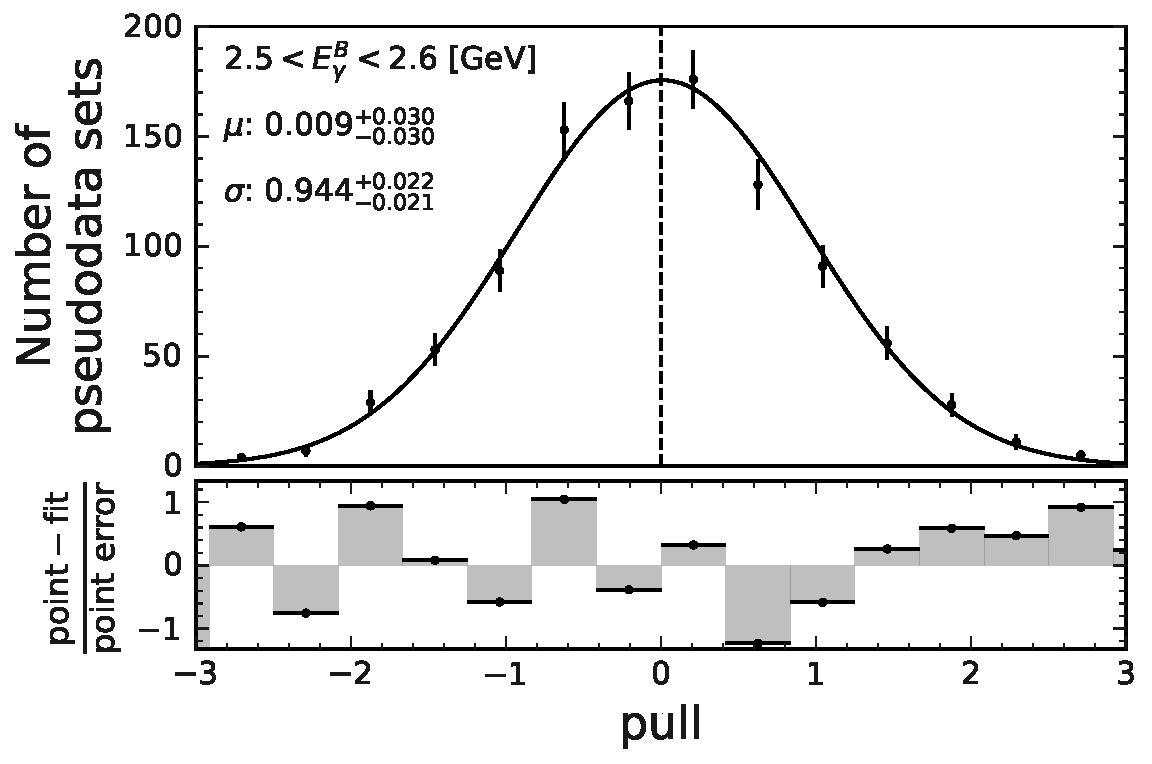
\includegraphics[width=0.22\textwidth]{figures/mc_validation/toy_study/fits_of_pulls_2p5to2p6.pdf}
    }
    \subcaptionbox{\label{fig:pulls_2p6to2p7}}{
        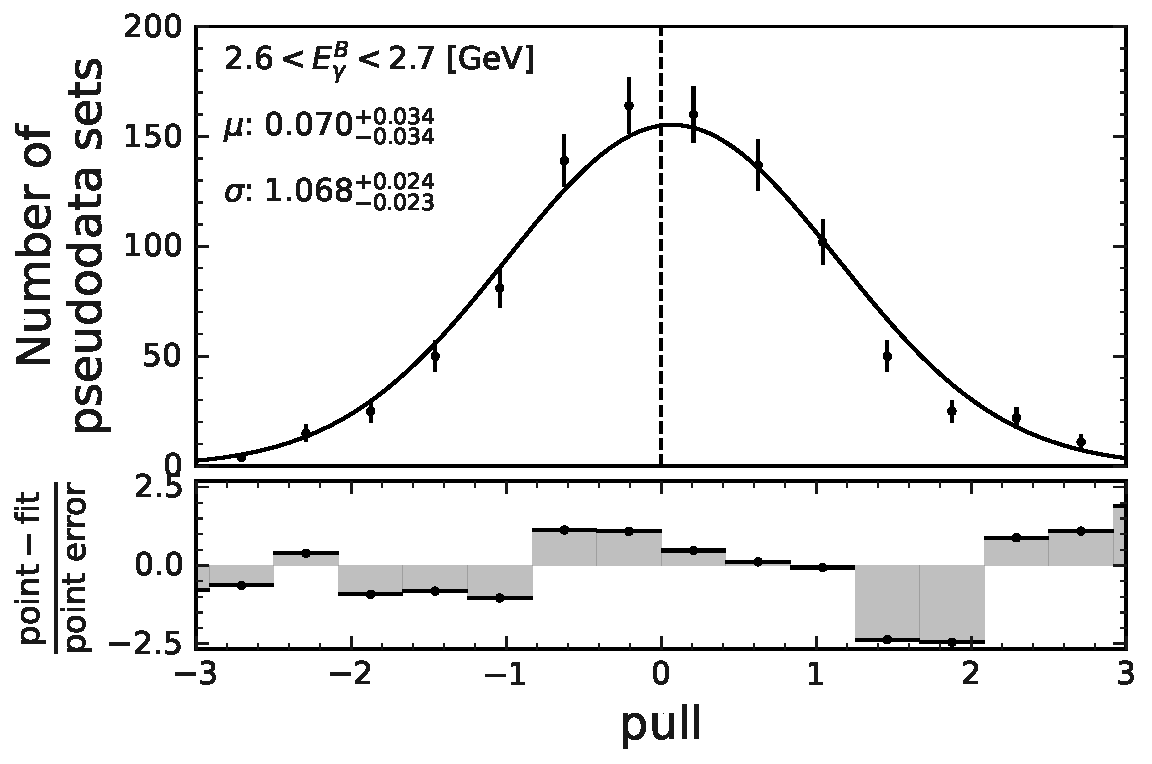
\includegraphics[width=0.22\textwidth]{figures/mc_validation/toy_study/fits_of_pulls_2p6to2p7.pdf}
    }
    \subcaptionbox{\label{fig:pulls_2p7to5p0}}{
        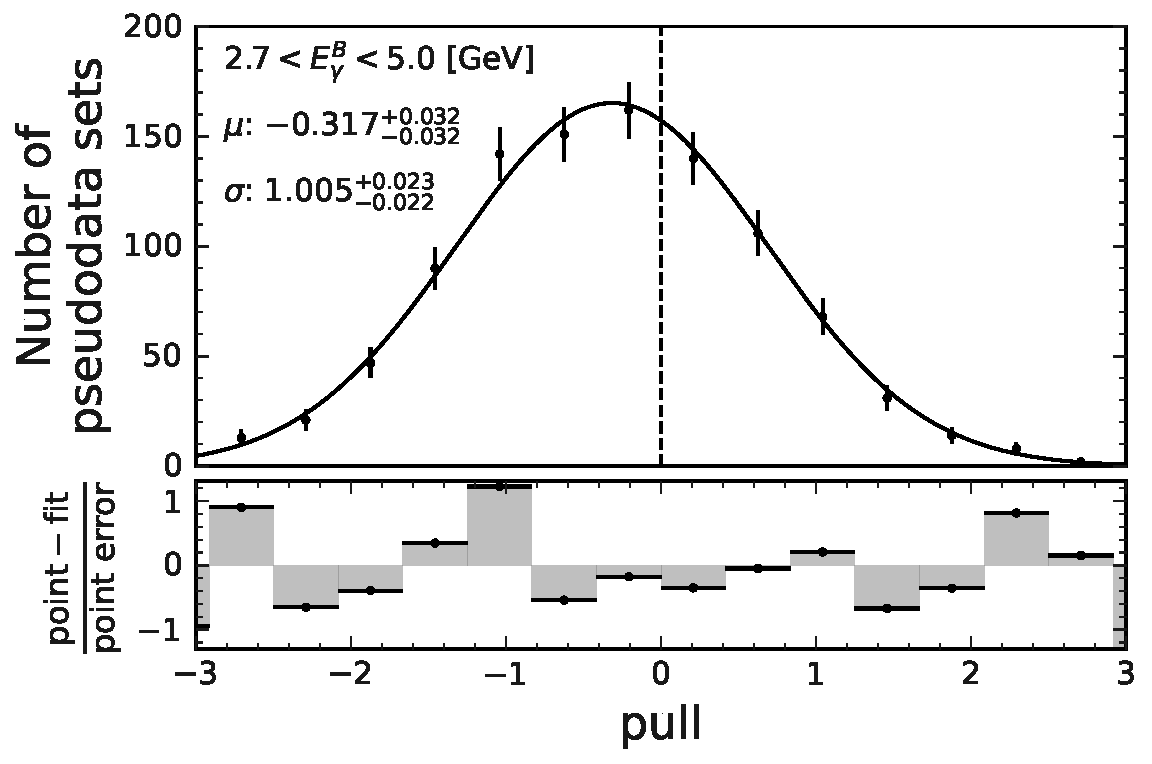
\includegraphics[width=0.22\textwidth]{figures/mc_validation/toy_study/fits_of_pulls_2p7to5p0.pdf}
    }
    \caption{\label{fig:pull_distributions}The pull distributions used in the \Mbc fitter closure test, 
    corresponding to results of 1000 pseudodata sets generated based on the \PDF fitted on the total generic \MC dataset.
    The definition of the pull, specifically for this test, is given in \Cref{eq:toy_pull}.
    The data points show the counts of values in the given pull intervals, and the uncertainty of each point is of statistical origin.
    The pulls are also fitted with a Gaussian distribution and the mean value, $\mu$, as well as the width, $sigma$, is also extracted.
    The fit is shown as a solid line, and is an unbinned fit (i.e. not the fit to the shown data points).
    }
\end{figure}

To test the statistical validity of \Mbc fits on each bin, a Gaussian \PDF is fitted on the distributions, with parameters $\mu$ and $\sigma$ being estimated.
The parameters correspond to the mean value, and the width of the Gaussian distribution, respectively.
The parameter estimation is performed as an unbinned negative log-likelihood fit.
The corresponding Gaussian fit results, and the parameters are shown in \Cref{fig:pull_distributions}, but also summarised neatly in \Cref{fig:mean_sigma_pulls}.

\begin{figure}[htbp!]
    \centering
    \subcaptionbox{\label{fig:mean_pulls}}{
        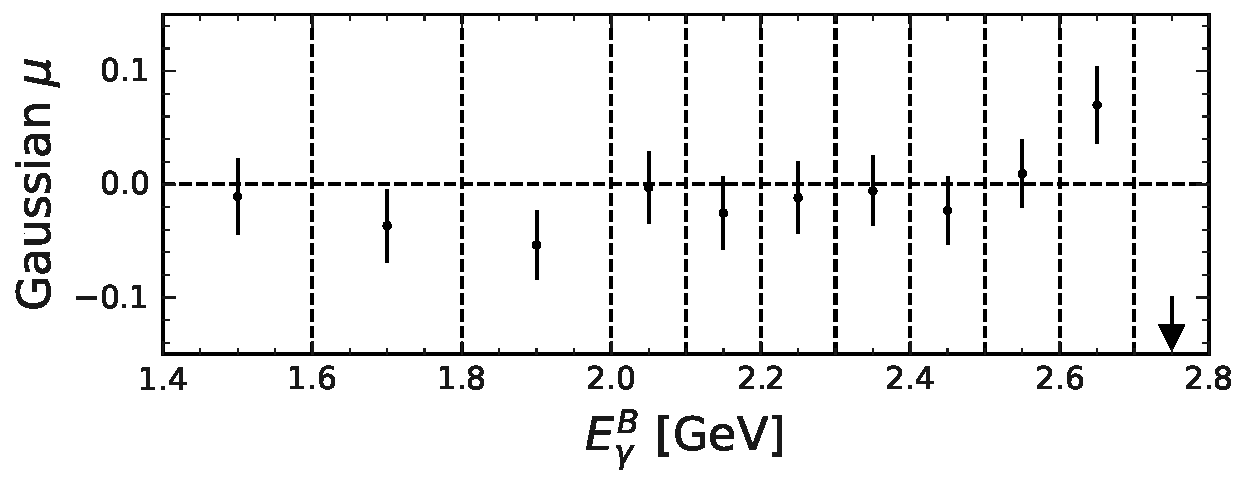
\includegraphics[width=0.4\textwidth]{figures/mc_validation/toy_study/mean_pull_toys.pdf}
    }
    \subcaptionbox{\label{fig:sigma_pulls}}{
        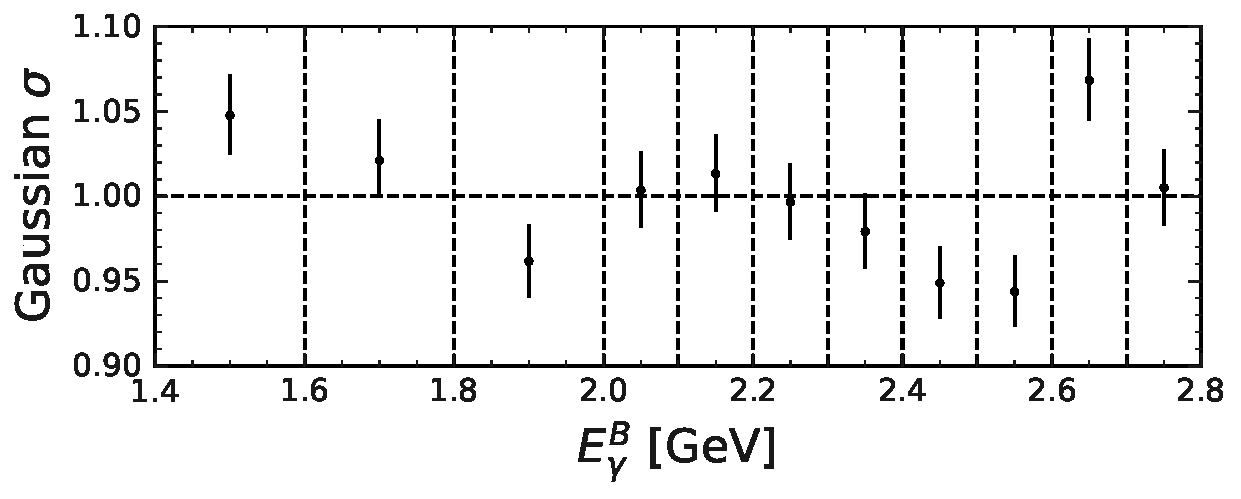
\includegraphics[width=0.4\textwidth]{figures/mc_validation/toy_study/sigma_pull_toys.pdf}
    }
    \caption{\label{fig:mean_sigma_pulls}Summarised means and widths ($\mu$ and $\sigma$, respectively) of the Gaussian fits of
    the pull distributions in each \EB bin.
    The fits for evaluation of $\mu$ and $\sigma$ are shown in \Cref{fig:pull_distributions}.
    The results are compatible with a unit Gaussian except in the case of parameter $\mu$ for $\EB>2.7~\gev$, where statistical effects play a large role.
    }
\end{figure}

The pulls are distributed as a Gaussian -- in all cases -- meaning that the central-limit theorem regime is reached.
It can also be seen that in all cases the results are compatible within up to 2 $\sigma$ with a unit Gaussian.
The only \EB bin where this is not true is the $\mu$ parameter in $\EB>2.7$.
Here, the central value of the pulls appear to be biased towards lower values.
This is attributed to statistical effects, as that bin has only a handful of entries (even at 1.6~\invab) therefore strongly affected by statistical background fluctuations.
As it is not expected to observe any statistically-significant signal events in that region, it is chosen to not define any correction based on the observed bias.

These results allow to conclude that the \Mbc fitter is an unbiased estimator.
In other words, the central values are unbiased and the uncertainties adequatly cover the Poissonian fluctuations of the results.

\subsection{Linearity test of the \texorpdfstring{\Mbc}{Mbc} fitter}\label{sec:linearity_test}

The fitter is further validated using the so-called \textit{linearity} test.
Any valid extended fit model ought to provide a behaviour such that the estimated normalisation, $\mathcal{N}$, grows linearly with the increase of the corresponding component in the fitted dataset.
To perform such a test in this analysis, up to 25000 \BtoXsgamma signal-\MC events where a good tag-\B meson has been identified are combined with the generic-\MC dataset.
For a valid fitting setup, $N$ events `injected' in the fitted dataset should yield approximately an increase of $N$ in the estimation $\mathcal{N}_{\mathrm{CB}}$.
Such test of the expected linear behaviour is summarised in \Cref{fig:linearity_test}.

\begin{figure}[htbp!]
    \centering
    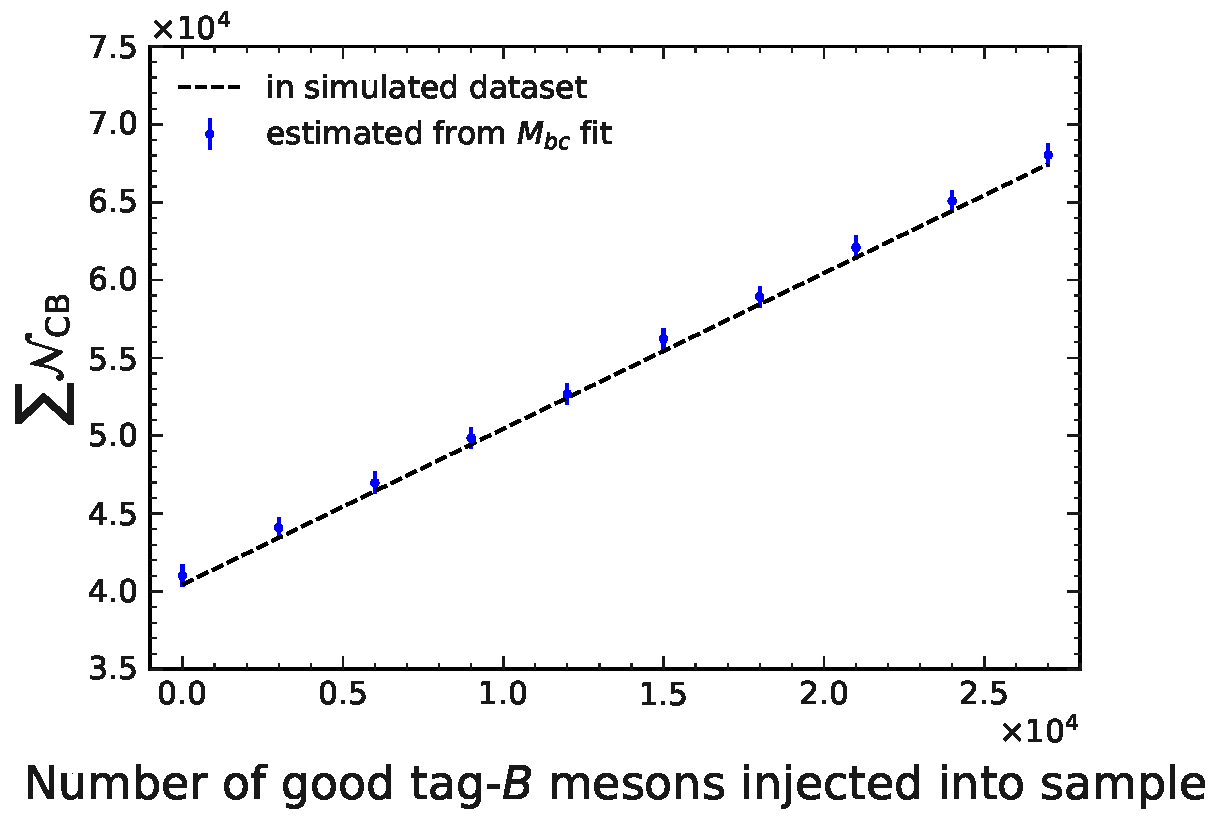
\includegraphics[width=0.45\textwidth]{figures/mc_validation/linearity_check_longer.pdf}
    \caption{\label{fig:linearity_test}The figure summarising the linearity test for the \Mbc fitter of this analysis.
    As the number of events, corresponding to the peaking tag-\B mesons increases, the extracted sum of normalisations across all bins, $\mathcal{N}_{\mathrm{CB}}$ also increases.
    The increase is compatible with a linear increase with a slope of 1.
    }
\end{figure}

As the number of `injected' good tag-\B events, the sum of the normalisations for all \EB bins should increase linearly.
This behaviour is clearly reproduced, as $\sum \mathcal{N}_{\mathrm{CB}}$ grows linearly with the increase of the dataset.
It can therefore be concluded that the behaviour of the \Mbc fitter is linear.

\subsection{Correlation matrix of the parameters of the \texorpdfstring{\Mbc}{Mbc} fitter}\label{sec:correlation_matrix}

Using the pseudodata sets generated in \Cref{sec:closure_test}, relationships between all parameters estimated by the \Mbc fitter can be calculated.
In particular, a correlation coefficient for some collection of paired values ${(x_1,y_1),(x_2,y_2,)...,(x_n,y_n)}$:
\begin{equation}\label{eq:pearson_r}
    R_{x,y}=\frac{\sum_{i=1}^n\left(x_i-\bar{x}\right)\left(y_i-\bar{y}\right)}{\sqrt{\sum_{i=1}^n\left(x_i-\bar{x}\right)^2} \sqrt{\sum_{i=1}^n\left(y_i-\bar{y}\right)^2}},
\end{equation}
which is called the Pearson-R coefficient.

For each two parameters estimated by the \Mbc fitter the Pearson-R value is evluated.
This results in a 36-by-36 matrix, corresponding to all parameters estimated by the \Mbc fitter in this analysis, and shown in \Cref{fig:correlation_matrix}.
The 37th parameter, $m_0$, is not included, because no significant correlations to that parameter are observed in the fitter.
\begin{figure}[htbp!]
    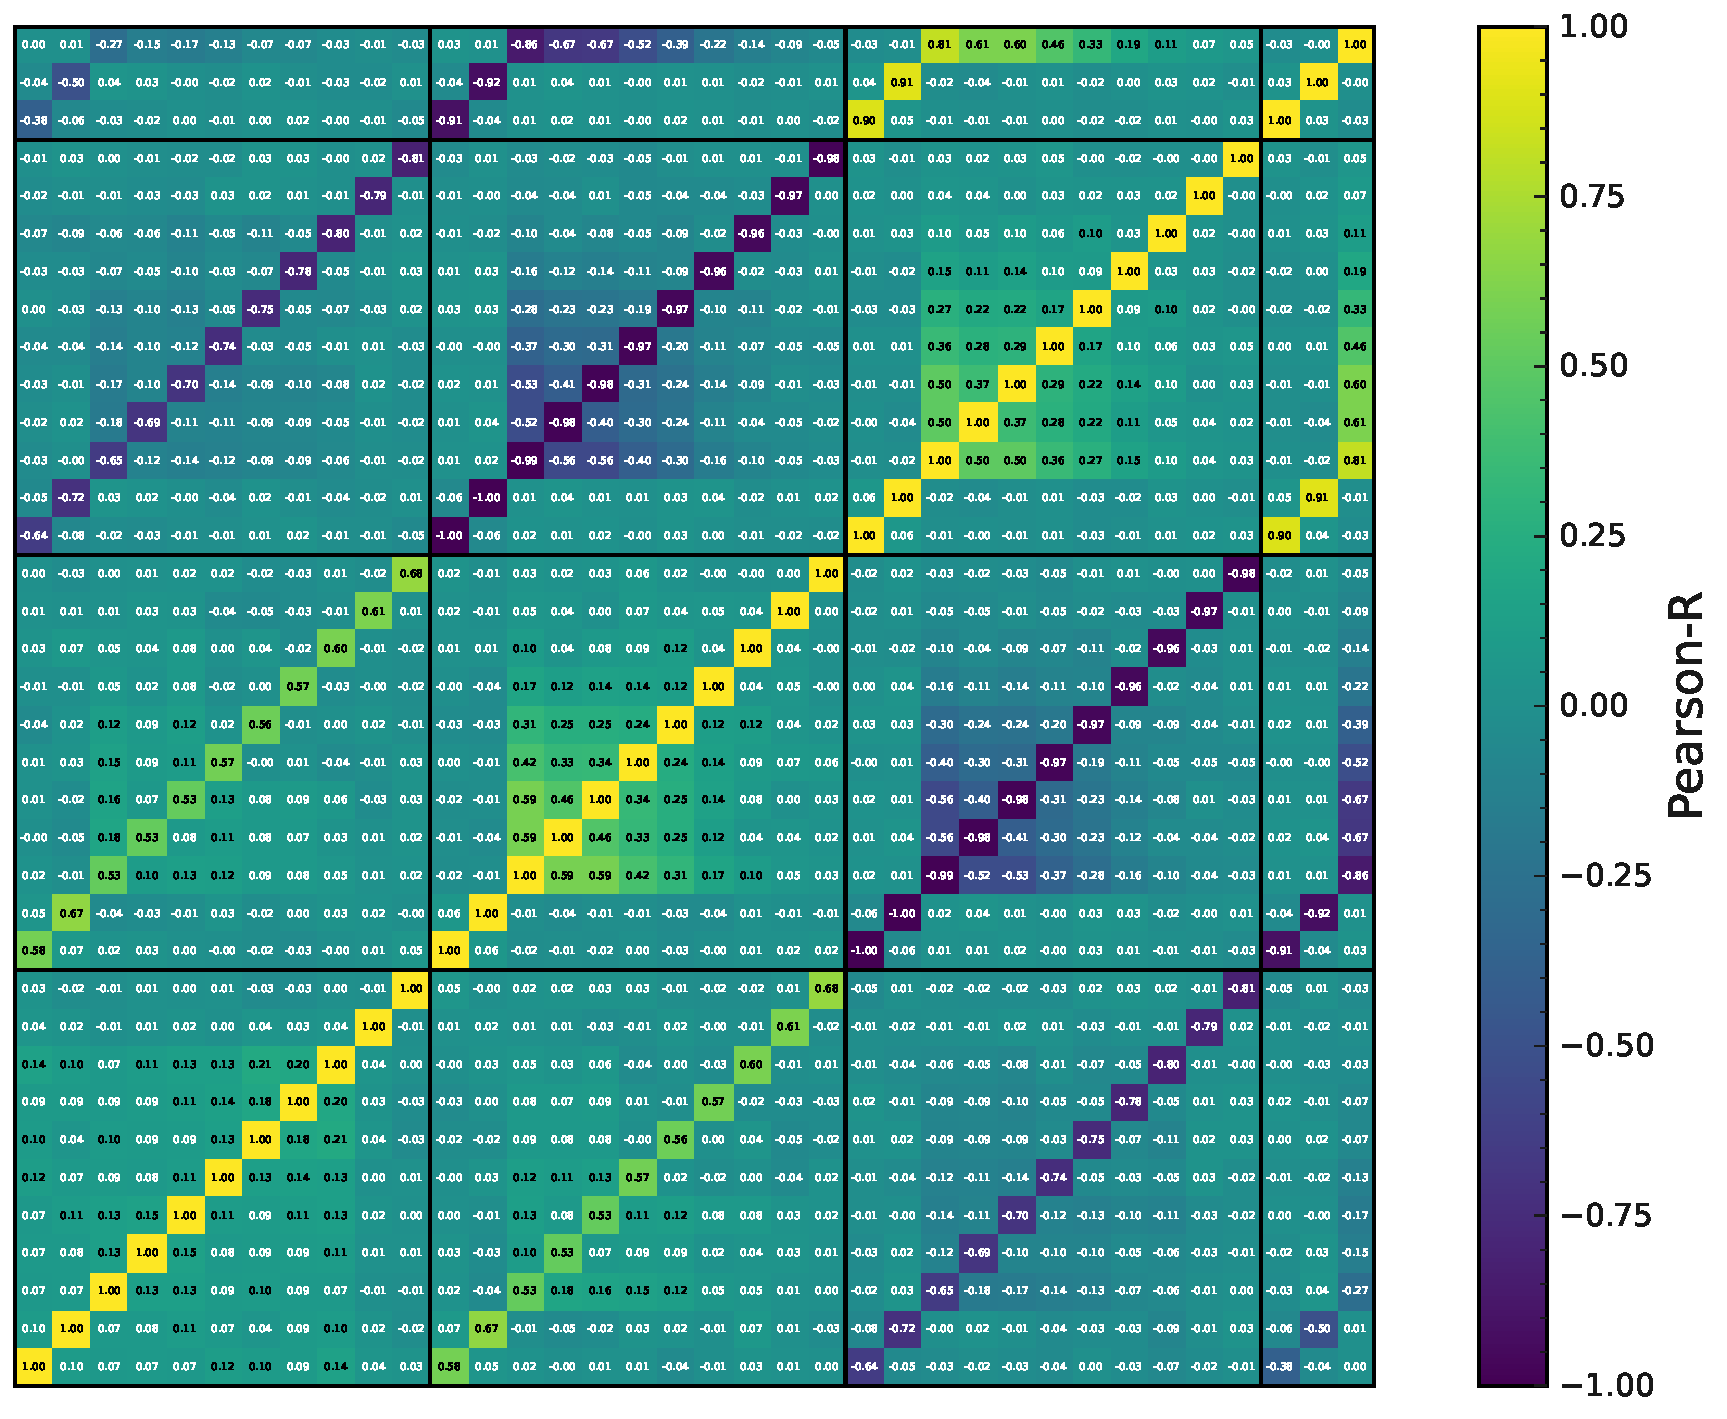
\includegraphics[width=1\textwidth]{figures/mc_validation/correlation_matrix.pdf}
    \caption{\label{fig:correlation_matrix}The correlation matrix of the \Mbc fitter, generated using a 1000 pseudodata set.
    Every pair of parameters has their correlation evaluates as the Pearson-R coefficient (\Cref{eq:pearson_r}).
    Parameter names correspond to those in \Cref{tab:fitting_init_params} and numbers $0-10$ correspond to the bin number, starting from $1.4-1.6~\gev$.
    }
\end{figure}

Several important insights into the fitter can be understood by observing the correlation matrix:
\begin{itemize}
\item
Firstly, consider the correlation of ${\mathcal{N}_{\mathrm{CB}}}_i$ with ${\mathcal{N}_{\mathrm{CB}}}_j$.
Clearly, the correlations are low -- implying that increases in one bin do not induce strong differences in other bins, as is to be expected.
Small correlations that can be observed are likely a combination of correlations through other parametrs (see later) and statistical fluctuations.
In general, most of the values are correlated by less than 10\%.
\item Secondly, consider the correlation of ${\mathcal{N}_{\mathrm{CB}}}_i$ with ${\mathcal{N}_{\mathrm{CHEB}}}_i$.
It can clearly be seen that the diagonal elements are strongly anti-correlated.
This is understood as a consequence of the fact that both Chebyshev and Crystal Ball \PDF{s} contain a degree of `peaking' behaviour in \Mbc.
Therefore, larger $\mathcal{N}_{\mathrm{CHEB}}$ values lead to lower ${\mathcal{N}_{\mathrm{CB}}}$, simply because the peaking behaviour of one parameter diminshed the other's.
\item Thirdly, consider the correlation of ${\mathcal{N}_{\mathrm{CB}}}_i$ with ${\mathcal{N}_{\mathrm{ARGUS}}}_i$.
This correlation is positive -- and understood as a direct result of the second point.
If the $\mathcal{N}_{\mathrm{CB}}$ is evaluated as larger, the Chebyshev polynomial, which is suppressed as a result, can also less adequatly describe the low-en of \Mbc.
That region must therefore be described by the $\mathcal{N}_{\mathrm{ARGUS}}$, inducing a chain of correlation: $\mathcal{N}_{\mathrm{CB}}\uparrow\rightarrow{\mathcal{N}_{\mathrm{CHEB}}}\downarrow\rightarrow\mathcal{N}_{\mathrm{ARGUS}}\uparrow$.
\item Fourthly, correlations of ${\mathcal{N}_{\mathrm{CB}}}_i$ with $c_j$.
This can be understood in a similar way as the correlation with ${\mathcal{N}_{\mathrm{CHEB}}}_i$.
The parameter $c$ controls the shape of the ARGUS \PDF{s}.
Notably, larger and positive values of $c$ tend to produce a \PDF that has more area at high-\Mbc than at low-\Mbc, producing, mimicking `peaking' behaviour.
Therefore largely negative values of $c$ introduce larger values of $\mathcal{N}_{\mathrm{CB}}$.
\item Finally, $\mathcal{N}_{\mathrm{CB}}$ correlations with off-diagonal elements of other parameters.
In these cases, the correlations are very small, similar like the ${\mathcal{N}_{\mathrm{CB}}}_{i,j}$ correlations, but they follow the trends of the diagonal elements.
This behaviour is interpreted through the effects of the shared parameter $c$.
As the parameter modified the shape of the total \PDF, these changes induce differences to $\mathcal{N}_{\mathrm{ARGUS}}$ which propagate as differences to other normalisation parameters, through discussed relations.
Particularly, because the variations of $c$ cause an increase to several bins simultaneously, correlations between off-diagonal elements ${\mathcal{N}_{\mathrm{CB}}}_{i,j}$ are also observed.
\end{itemize}

A study with more than 1000 pseudodata sets may be necessary in the future to better understand the indirect off-bin correlations present in this analysis.
As correlations for ${\mathcal{N}_{\mathrm{CB}}}_{i,j}$ are observed as small and indirect, they are not considered to significantly affect the result in this analysis.
Therefore, it is concluded that no unexpected behaviour of the fitter is observed, with correlations between different parameters explainable through the differences in the \PDF shape they introduce.
